
\par The selections and analysis described below rely on well understood detector, simulation, calibration, and analysis tools performance. This section is dedicated to evaluating the performance of detector modeling through data-mc comparisons of targeted samples. The sidebands developed for this analysis are a high-stats $\pi^0$ selection, and an \emph{anti-BDT} filter which targets the selection of $\nu_e$ like backgrounds. \emph{Currently comparisons for the \emph{anti-BDT} filter are not available and will be documented in a future iteration of this note.}
\par It is important to note that in addition to detector simulation and reconstruction effects, $\nu$-Ar modeling can impact the level of data-mc agreement in various variables. We will try to point out when this might be the case.
\subsection{$\pi^0$ control sample}
\label{sec:controls:pi0}
\par A $\pi^0$ selection has been developed in order to obtain high-stats samples of $\pi^0$ events and $\gamma$ EM showers which can constrain $\pi^0$ production modeling uncertainties as well as validate the analyis' ability to reconstruct and select EM showers.
\par Figure~\ref{fig:pi0:mass} shows the reconstructed di-photon mass (\texttt{M$\gamma\gamma$}) for candidate $\pi^0$ events, with a calibrated but uncorrected \footnote{With the term ``uncorrected", we mean that we do not account for biases in shower energy reconstruction caused by the incompleteness in charge clustering.} energy reconstruction. Overall, there is good data-MC agreement in shape, apart from an apparent normalization difference. To account for this normalization difference, we measure the flat scaling factor  for CC and NC $\pi^0$ events needed to obtain  a consistent rate in data and MC: this factor is 72.4\% in Run1 and 72.7\% in Run3. We repeat the exercise applying a tighter $\pi^0$ selection enhancing the $\pi^0$ purity and obtain scaling factors of 70\% for both Run1 and Run3. While this procedure is far from rigorous, it allows us to study detector-related and specifically shower-related variables removing a large normalization difference. \emph{A more rigorous data-driven constrain of our $\pi^0$ rate, performed accounting for detector and flux systematics, and considering a broader range of $\pi^0$ modeling, will need to be performed.}

\begin{figure}[H] 
\begin{center}
    \begin{subfigure}[b]{0.3\textwidth}
    \centering
    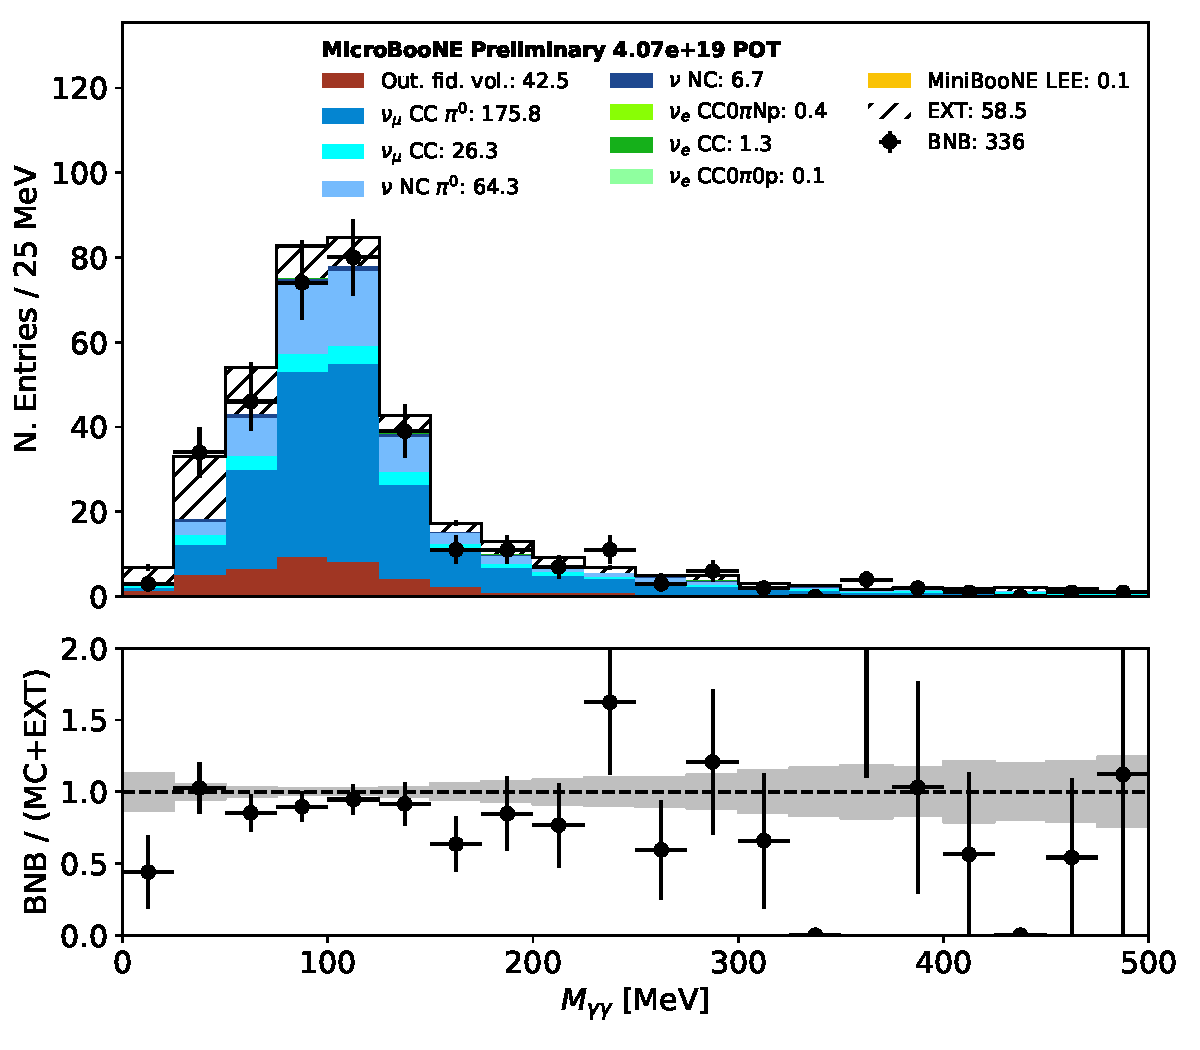
\includegraphics[width=1.00\textwidth]{pi0/pi0_mass_Y_01142020_5E19.pdf}
    \caption{\label{fig:pi0:mass:5E19} Run 1 ``5E19'' open dataset.}
    \end{subfigure}
    \begin{subfigure}[b]{0.3\textwidth}
    \centering
    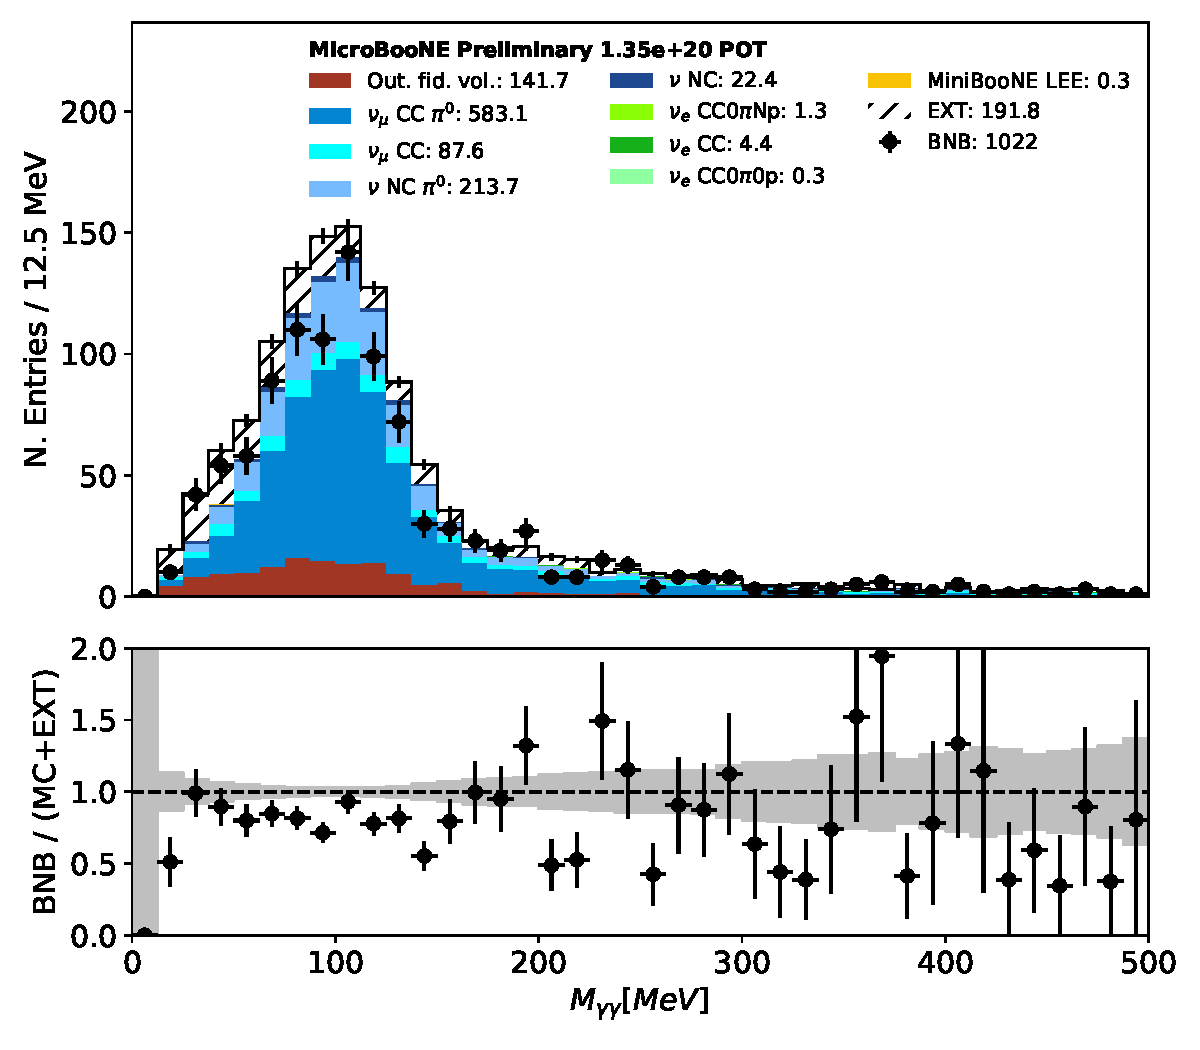
\includegraphics[width=1.00\textwidth]{pi0/pi0_mass_Y_01142020sel__RUN1.pdf}
    \caption{\label{fig:pi0:mass:5E19} Run 1.}
    \end{subfigure}
    \begin{subfigure}[b]{0.3\textwidth}
    \centering
    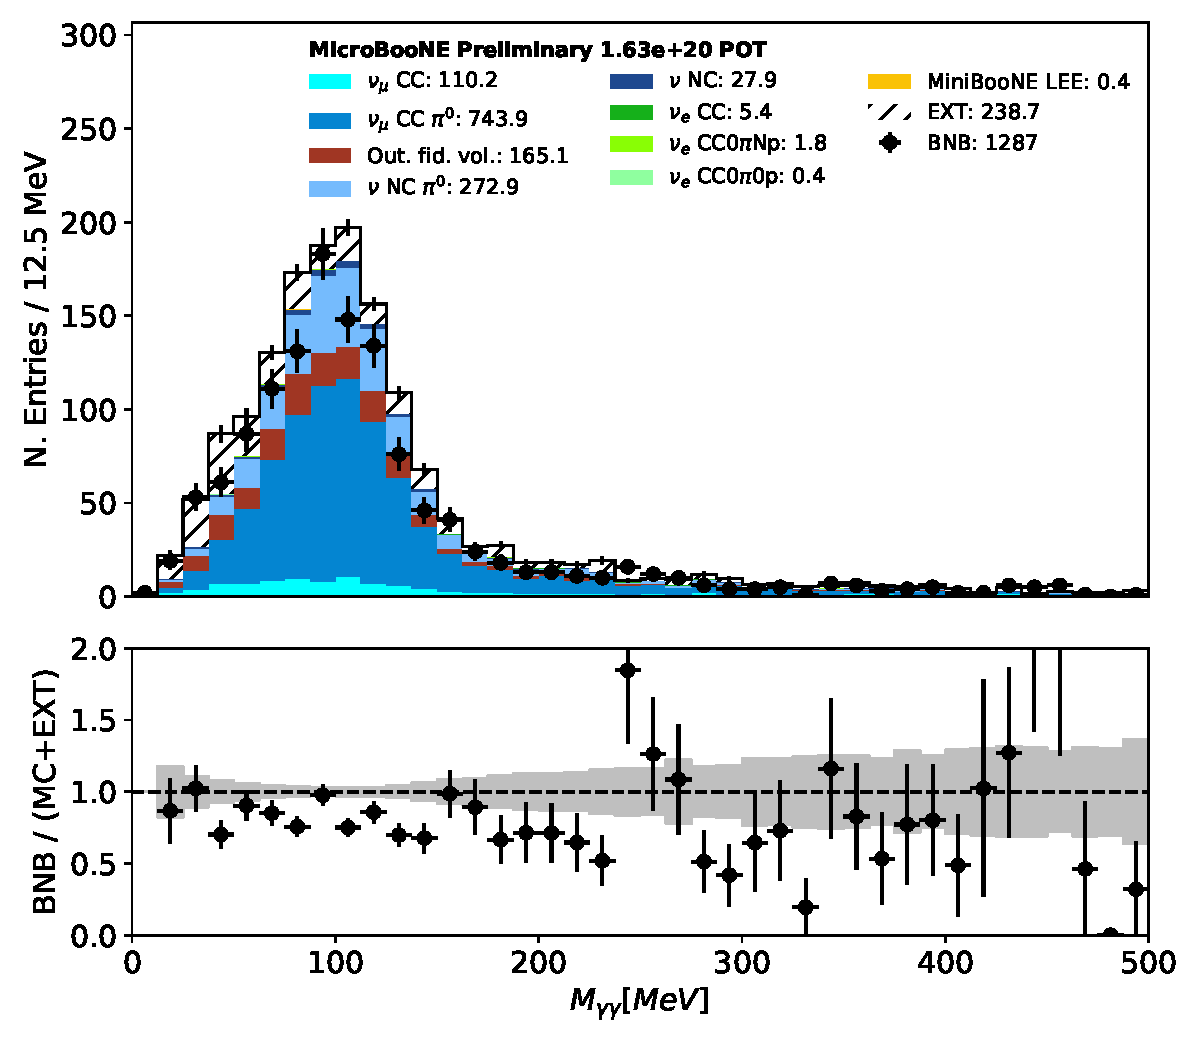
\includegraphics[width=1.00\textwidth]{pi0/pi0_mass_Y_01142020sel_RUN3.pdf}
    \caption{\label{fig:pi0:mass:5E19} Run 3.}
    \end{subfigure}
\caption{\label{fig:pi0:mass}Reconstructed $\pi^0$ mass.}
\end{center}
\end{figure}

\par After applying a scaling factor of 0.7 to CC and NC $\pi^0$ events in the MC, we show comparisons of shower variables with the goal of assessing data-mc agreement for the $\nu_e$ selection. Figure~\ref{fig:pi0:datamc} shows reconstructed quantities used in the $\nu_e$ analysis for $\pi^0$ candidate events which are useful in validating the robustness of shower modeling. They include leading and sub-leading shower dE/dx (top), followed by the leading and sub-leading shower conversion distance and shower score. The last row reports the reconstructed shower Moliere angle and track PID score for the longest track in each event. Generally, the data-MC agreement is quite good. For d$E$/d$x$ there appears to be a one bin shift to the left in data, specifically in the 4 MeV/cm peak associated with photons (see figure~\ref{fig:pi0:datamc} top-left). \emph{A re-calibration of shower d$E$/d$x$ is planned for the analysis, but has not been fully implemented at the moment.}

\begin{figure}[H] 
\begin{center}
    \begin{subfigure}[b]{0.38\textwidth}
    \centering
    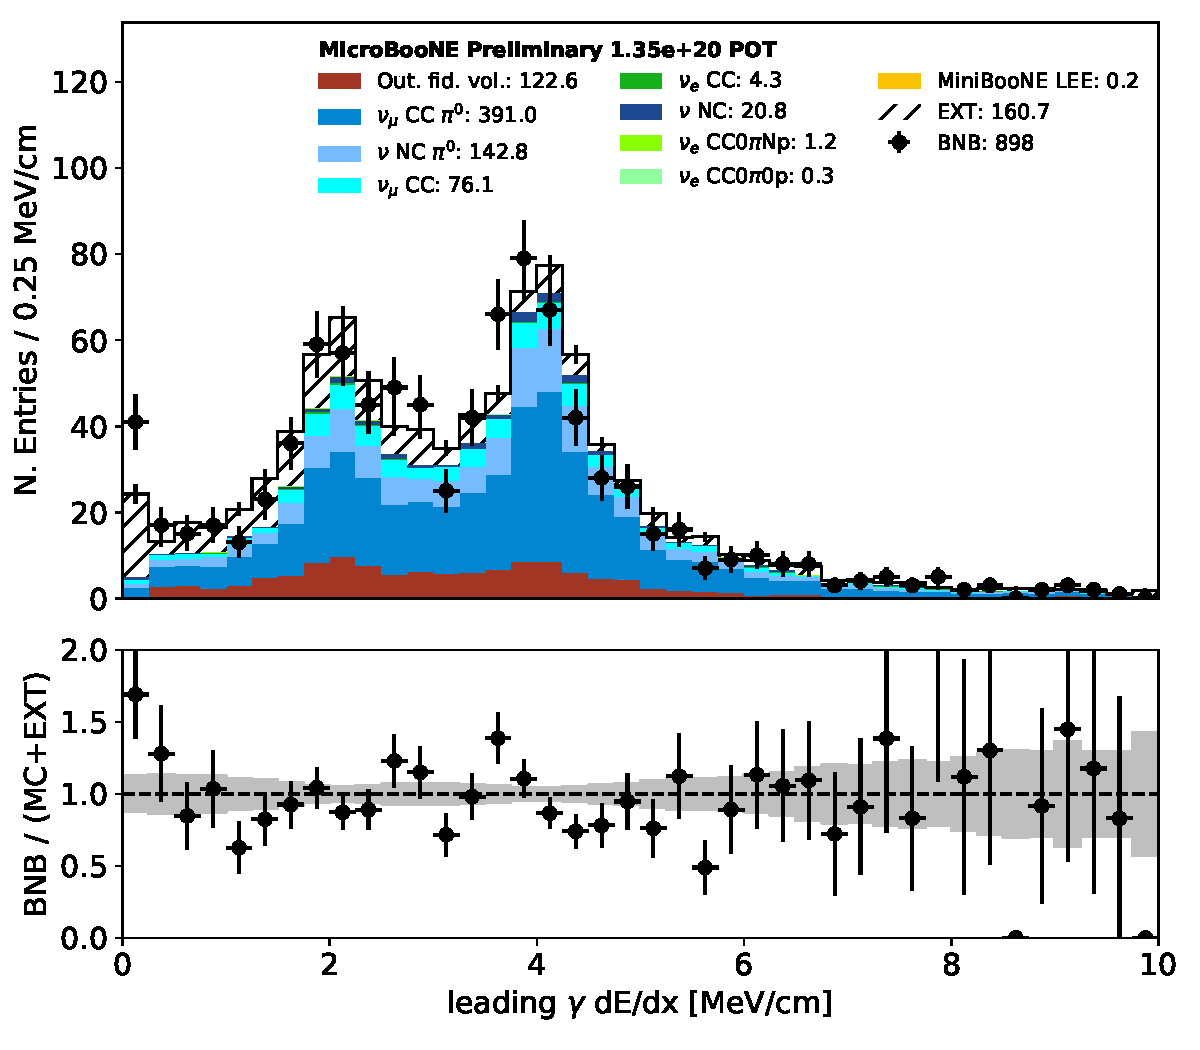
\includegraphics[width=1.00\textwidth]{pi0/pi0_dedx1_fit_Y_01152020_scaled_RUN1.pdf}
    %\caption{\label{fig:pi0:dedx:RUN1:leading} Run 1 leading shower.}
    \end{subfigure}
    \begin{subfigure}[b]{0.38\textwidth}
    \centering
    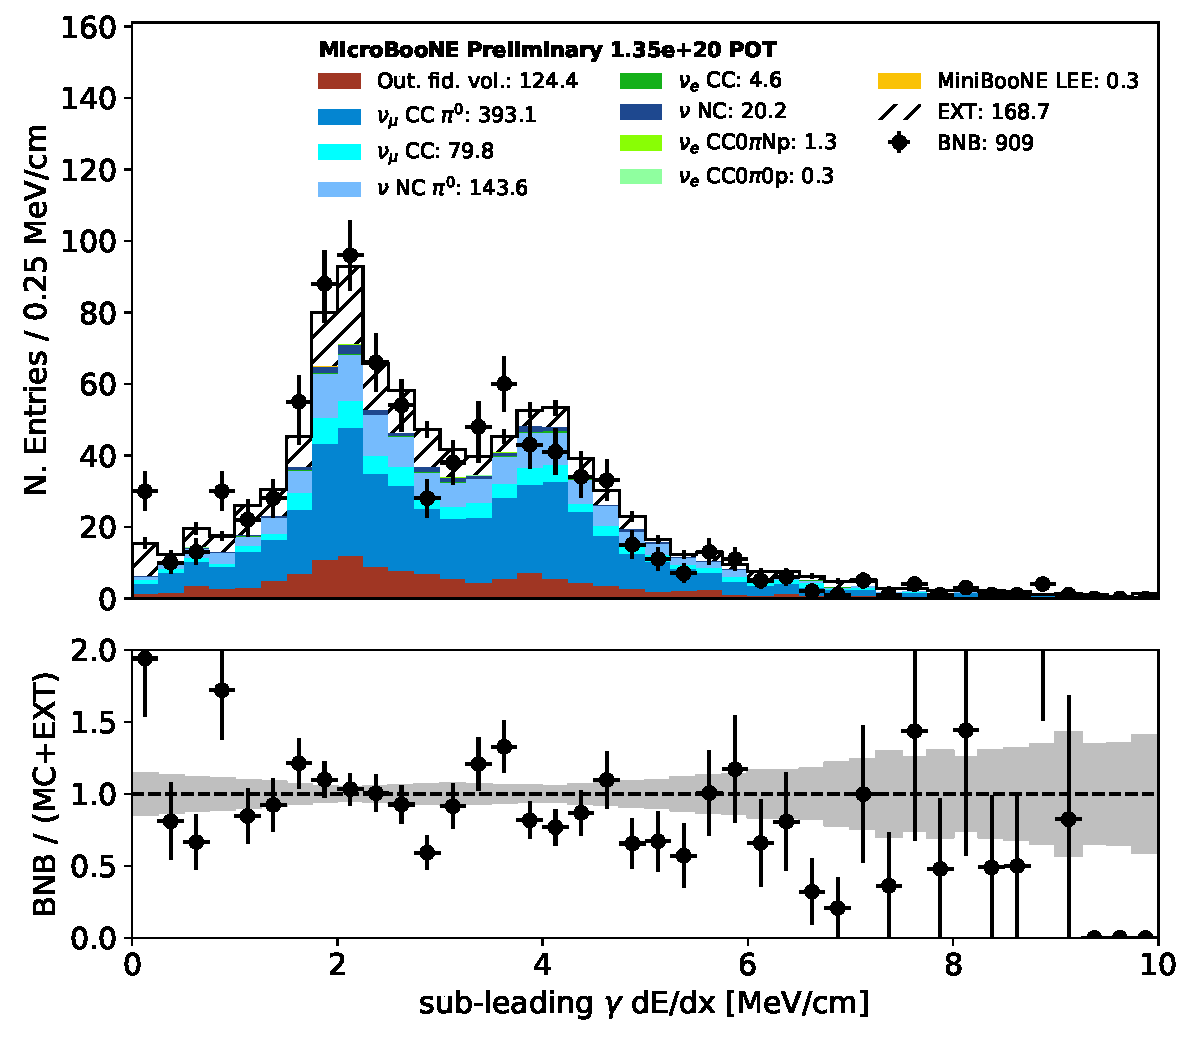
\includegraphics[width=1.00\textwidth]{pi0/pi0_dedx2_fit_Y_01152020_scaled_RUN1.pdf}
    %\caption{\label{fig:pi0:dedx:RUN1:subleading} Run 1 sub-leading shower.}
    \end{subfigure}
    
    \begin{subfigure}[b]{0.38\textwidth}
    \centering
    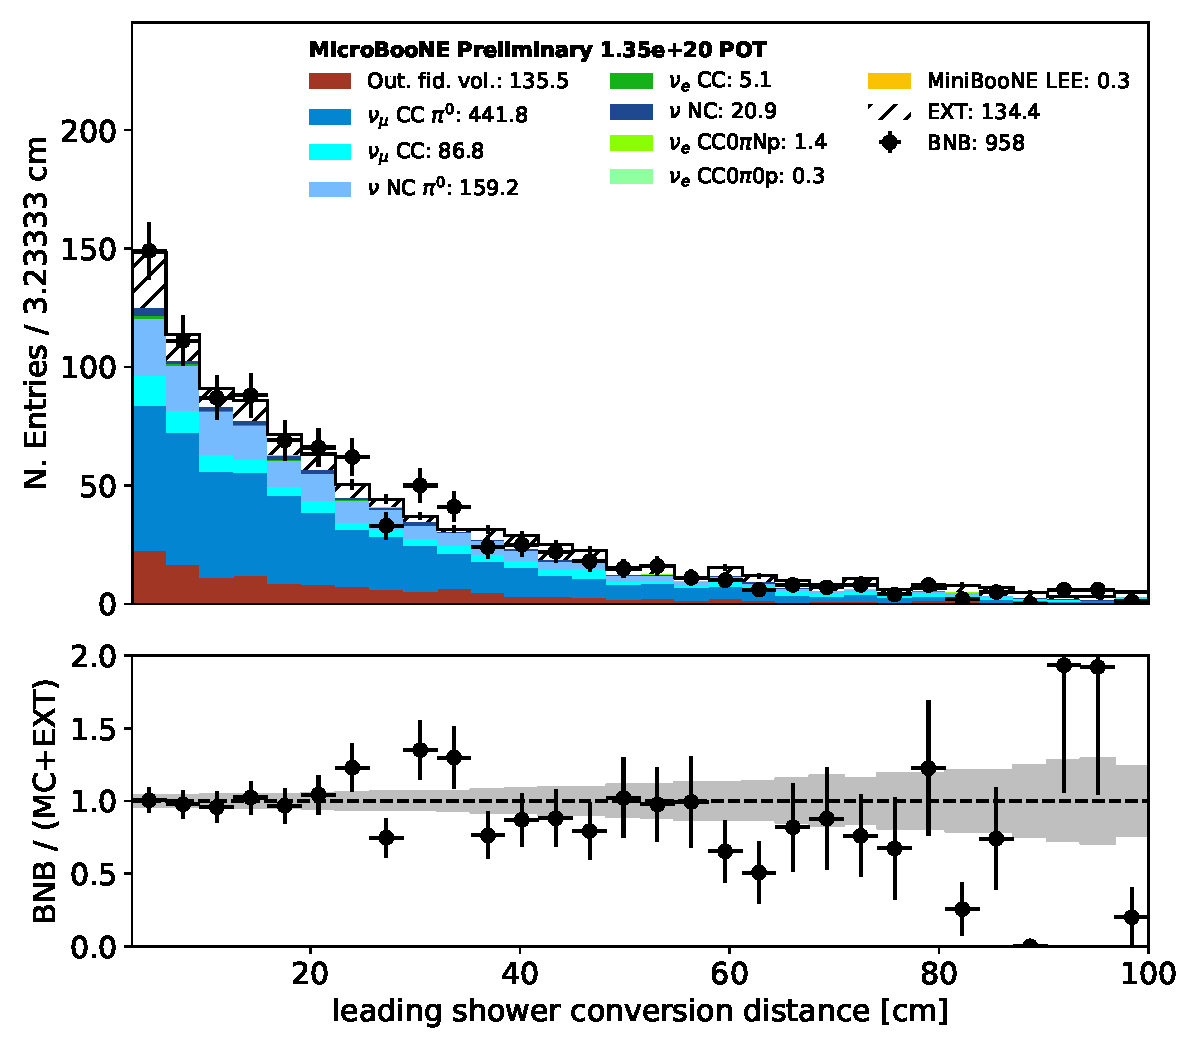
\includegraphics[width=1.00\textwidth]{pi0/pi0_radlen1_01152020_inputs_RUN1.pdf}
    %\caption{\label{fig:pi0:dedx:RUN1:leading} Run 1 leading shower.}
    \end{subfigure}
    \begin{subfigure}[b]{0.38\textwidth}
    \centering
    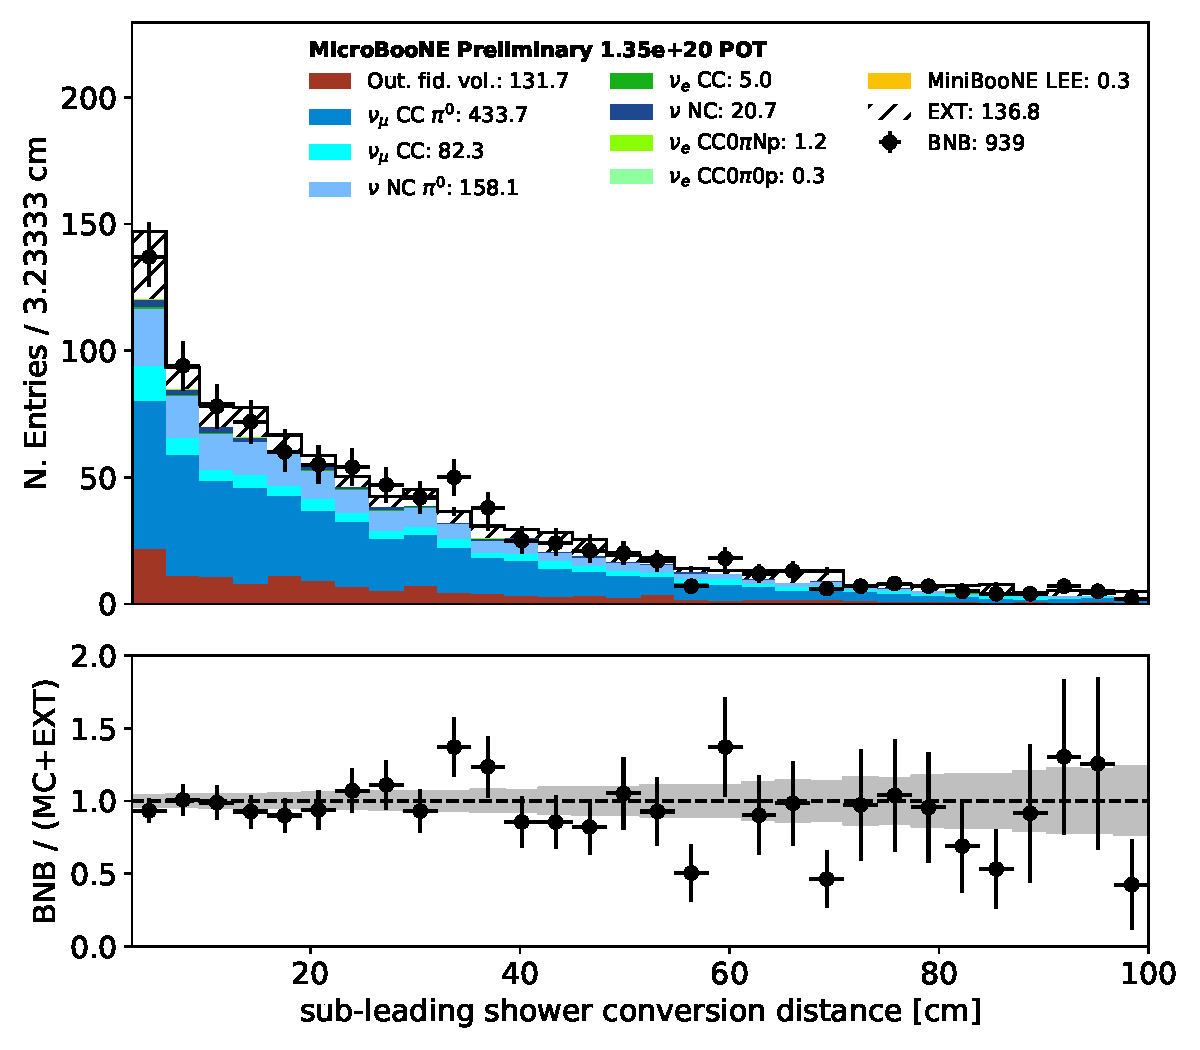
\includegraphics[width=1.00\textwidth]{pi0/pi0_radlen2_01152020_inputs_RUN1.pdf}
    %\caption{\label{fig:pi0:dedx:RUN1:subleading} Run 1 sub-leading shower.}
    \end{subfigure}
    
    \begin{subfigure}[b]{0.38\textwidth}
    \centering
    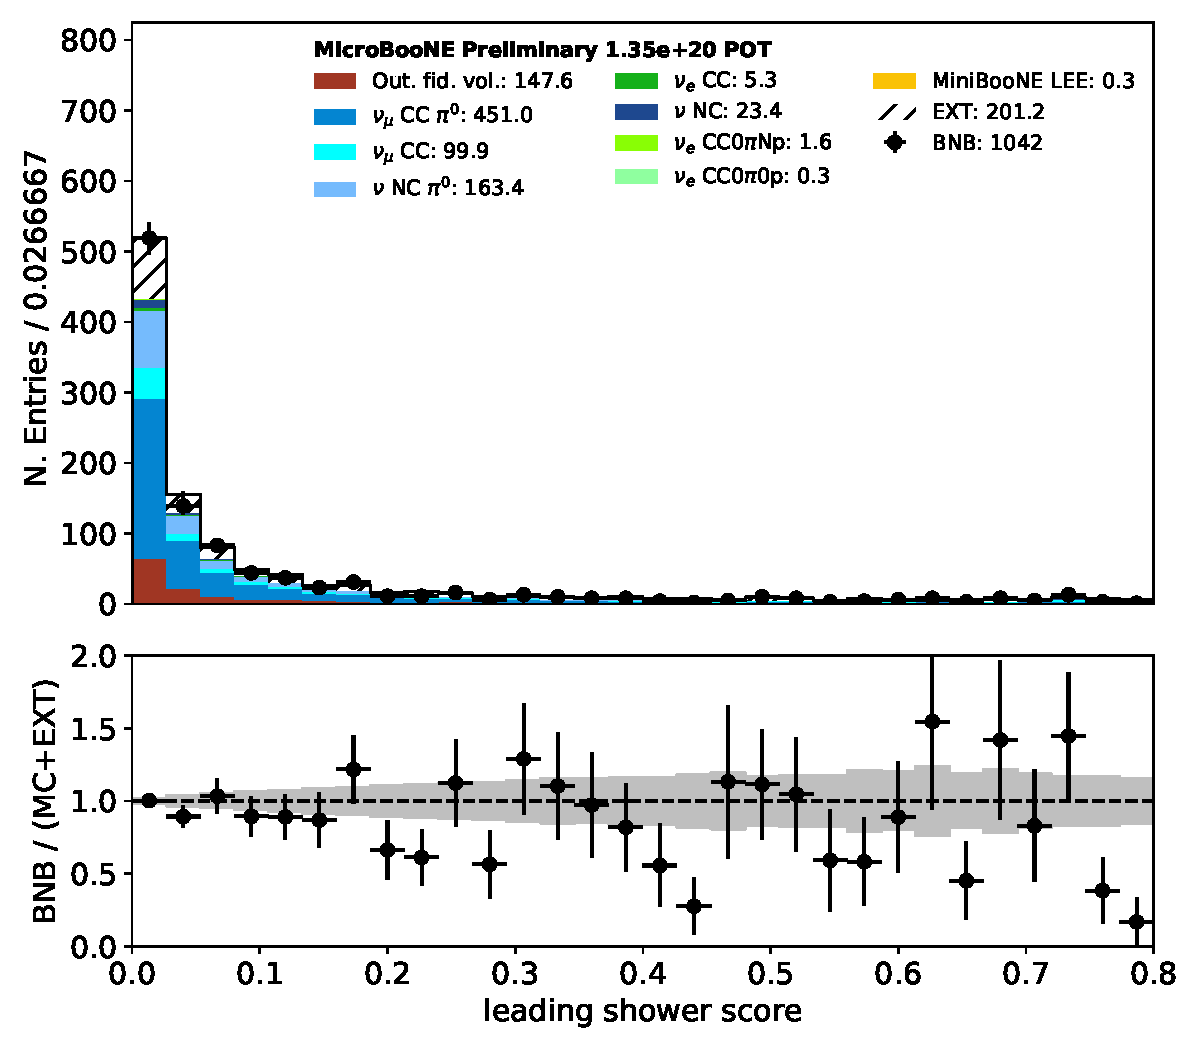
\includegraphics[width=1.00\textwidth]{pi0/pi0_shrscore1_01152020_inputs_RUN1.pdf}
    %\caption{\label{fig:pi0:dedx:RUN1:leading} Run 1 leading shower.}
    \end{subfigure}
    \begin{subfigure}[b]{0.38\textwidth}
    \centering
    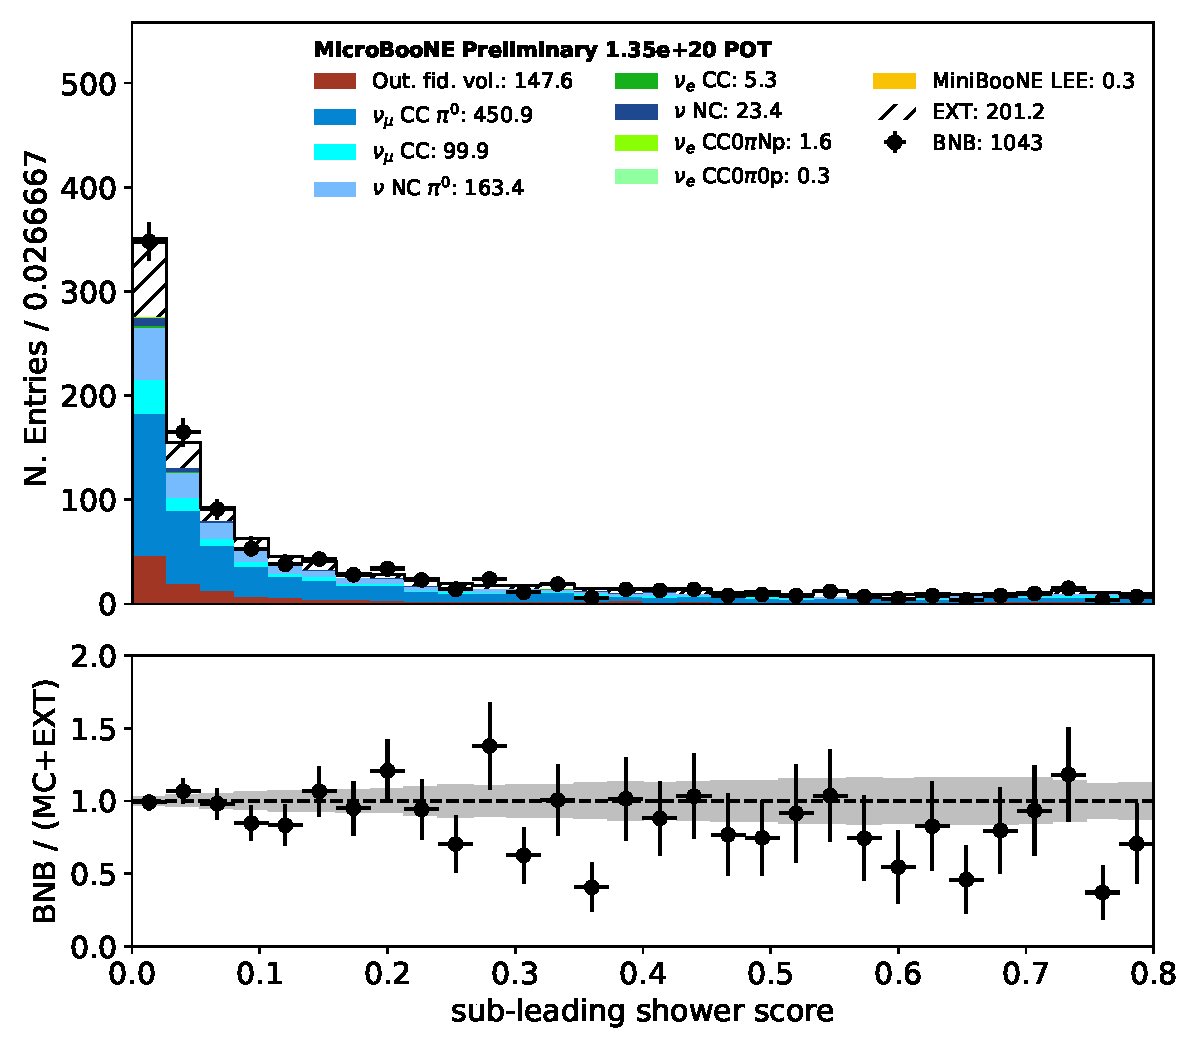
\includegraphics[width=1.00\textwidth]{pi0/pi0_shrscore2_01152020_inputs_RUN1.pdf}
    %\caption{\label{fig:pi0:dedx:RUN1:subleading} Run 1 sub-leading shower.}
    \end{subfigure}
    
    \begin{subfigure}[b]{0.38\textwidth}
    \centering
    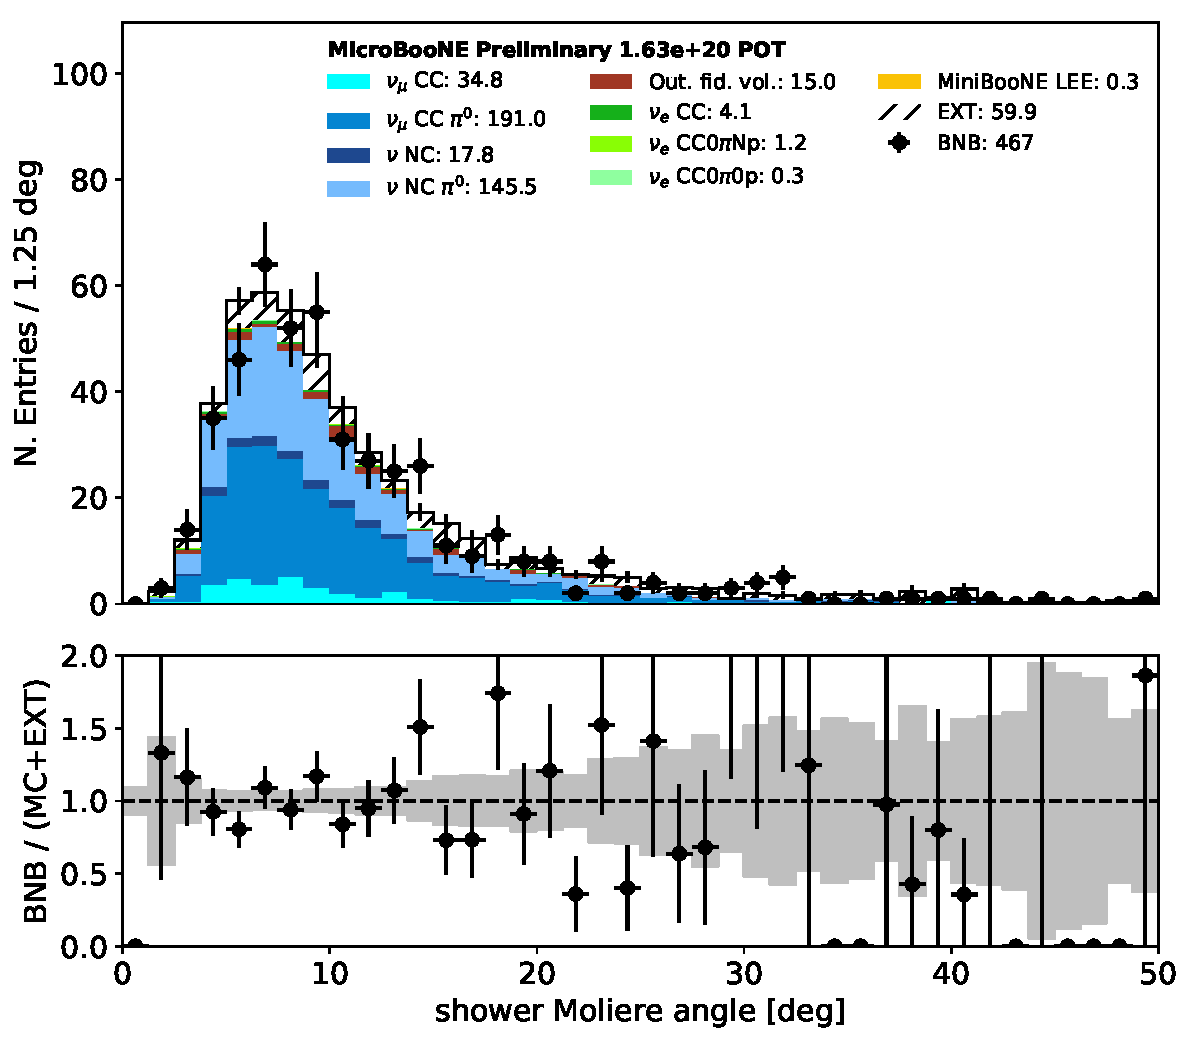
\includegraphics[width=1.00\textwidth]{pi0/shrmoliereavg_01152020_scaled_RUN3.pdf}
    %\caption{\label{fig:pi0:dedx:RUN1:leading} Run 1 leading shower.}
    \end{subfigure}
    \begin{subfigure}[b]{0.38\textwidth}
    \centering
    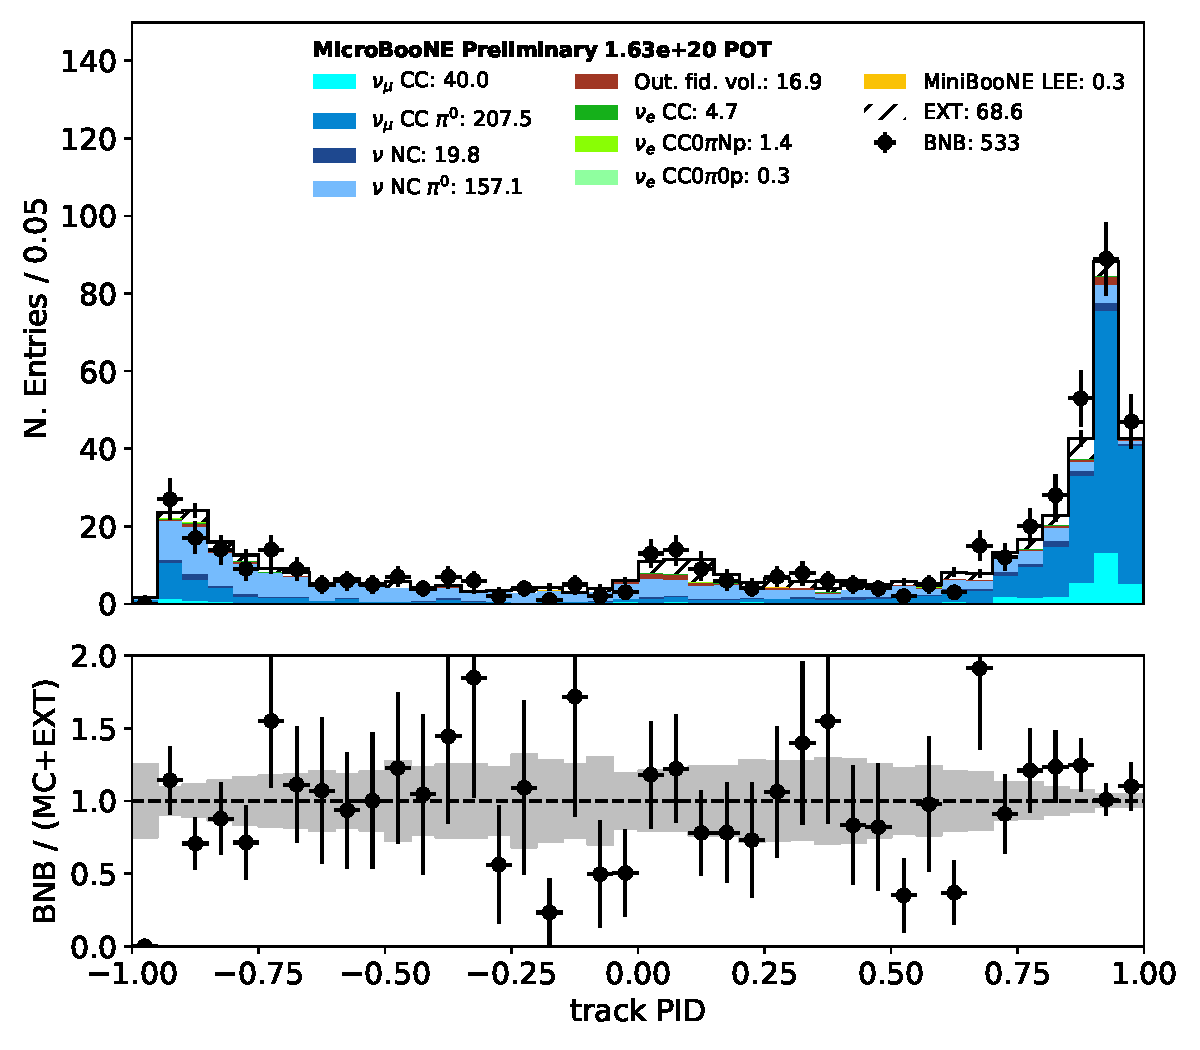
\includegraphics[width=1.00\textwidth]{pi0/trkpid_01152020_scaled_RUN3.pdf}
    %\caption{\label{fig:pi0:dedx:RUN1:subleading} Run 1 sub-leading shower.}
    \end{subfigure}
    
\caption{\label{fig:pi0:datamc}Reconstructed d$E$/d$x$ for leading and sub-leading showers.}
\end{center}
\end{figure}

\subsection{Anti-BDT sample}
\par An anti-BDT filter was developed with the goal of isolating $\nu_e$ like backgrounds that could help study in detail data-mc agreement for events that are close to, but not in the $\nu_e$ signal region. The filter selects events that pass the $\nu_e$  pre-selection but fail a past iteration of the 1$e$N$p$ BDT, in order to veto and remain blind to signal events. The filter was run on $1.5E20$ POT of Run 3 data with the goal of studying in particular detail data-mc agreement for Run3, which otherwise would be limited to $0.8E19$ POT of open data. Further documentation on the \emph{anti-BDT} filter is available in reference~\cite{bib:antiBDT}. \emph{Comparisons of distributions from this filter are to be made available in a subsequent version of this note.}
